\section{\absmachine: An abstract machine for programmable switches}
\label{s:absmachine}

%TODO: Say somewhere that all references to state are switch state.

\begin{figure*}[!t]
  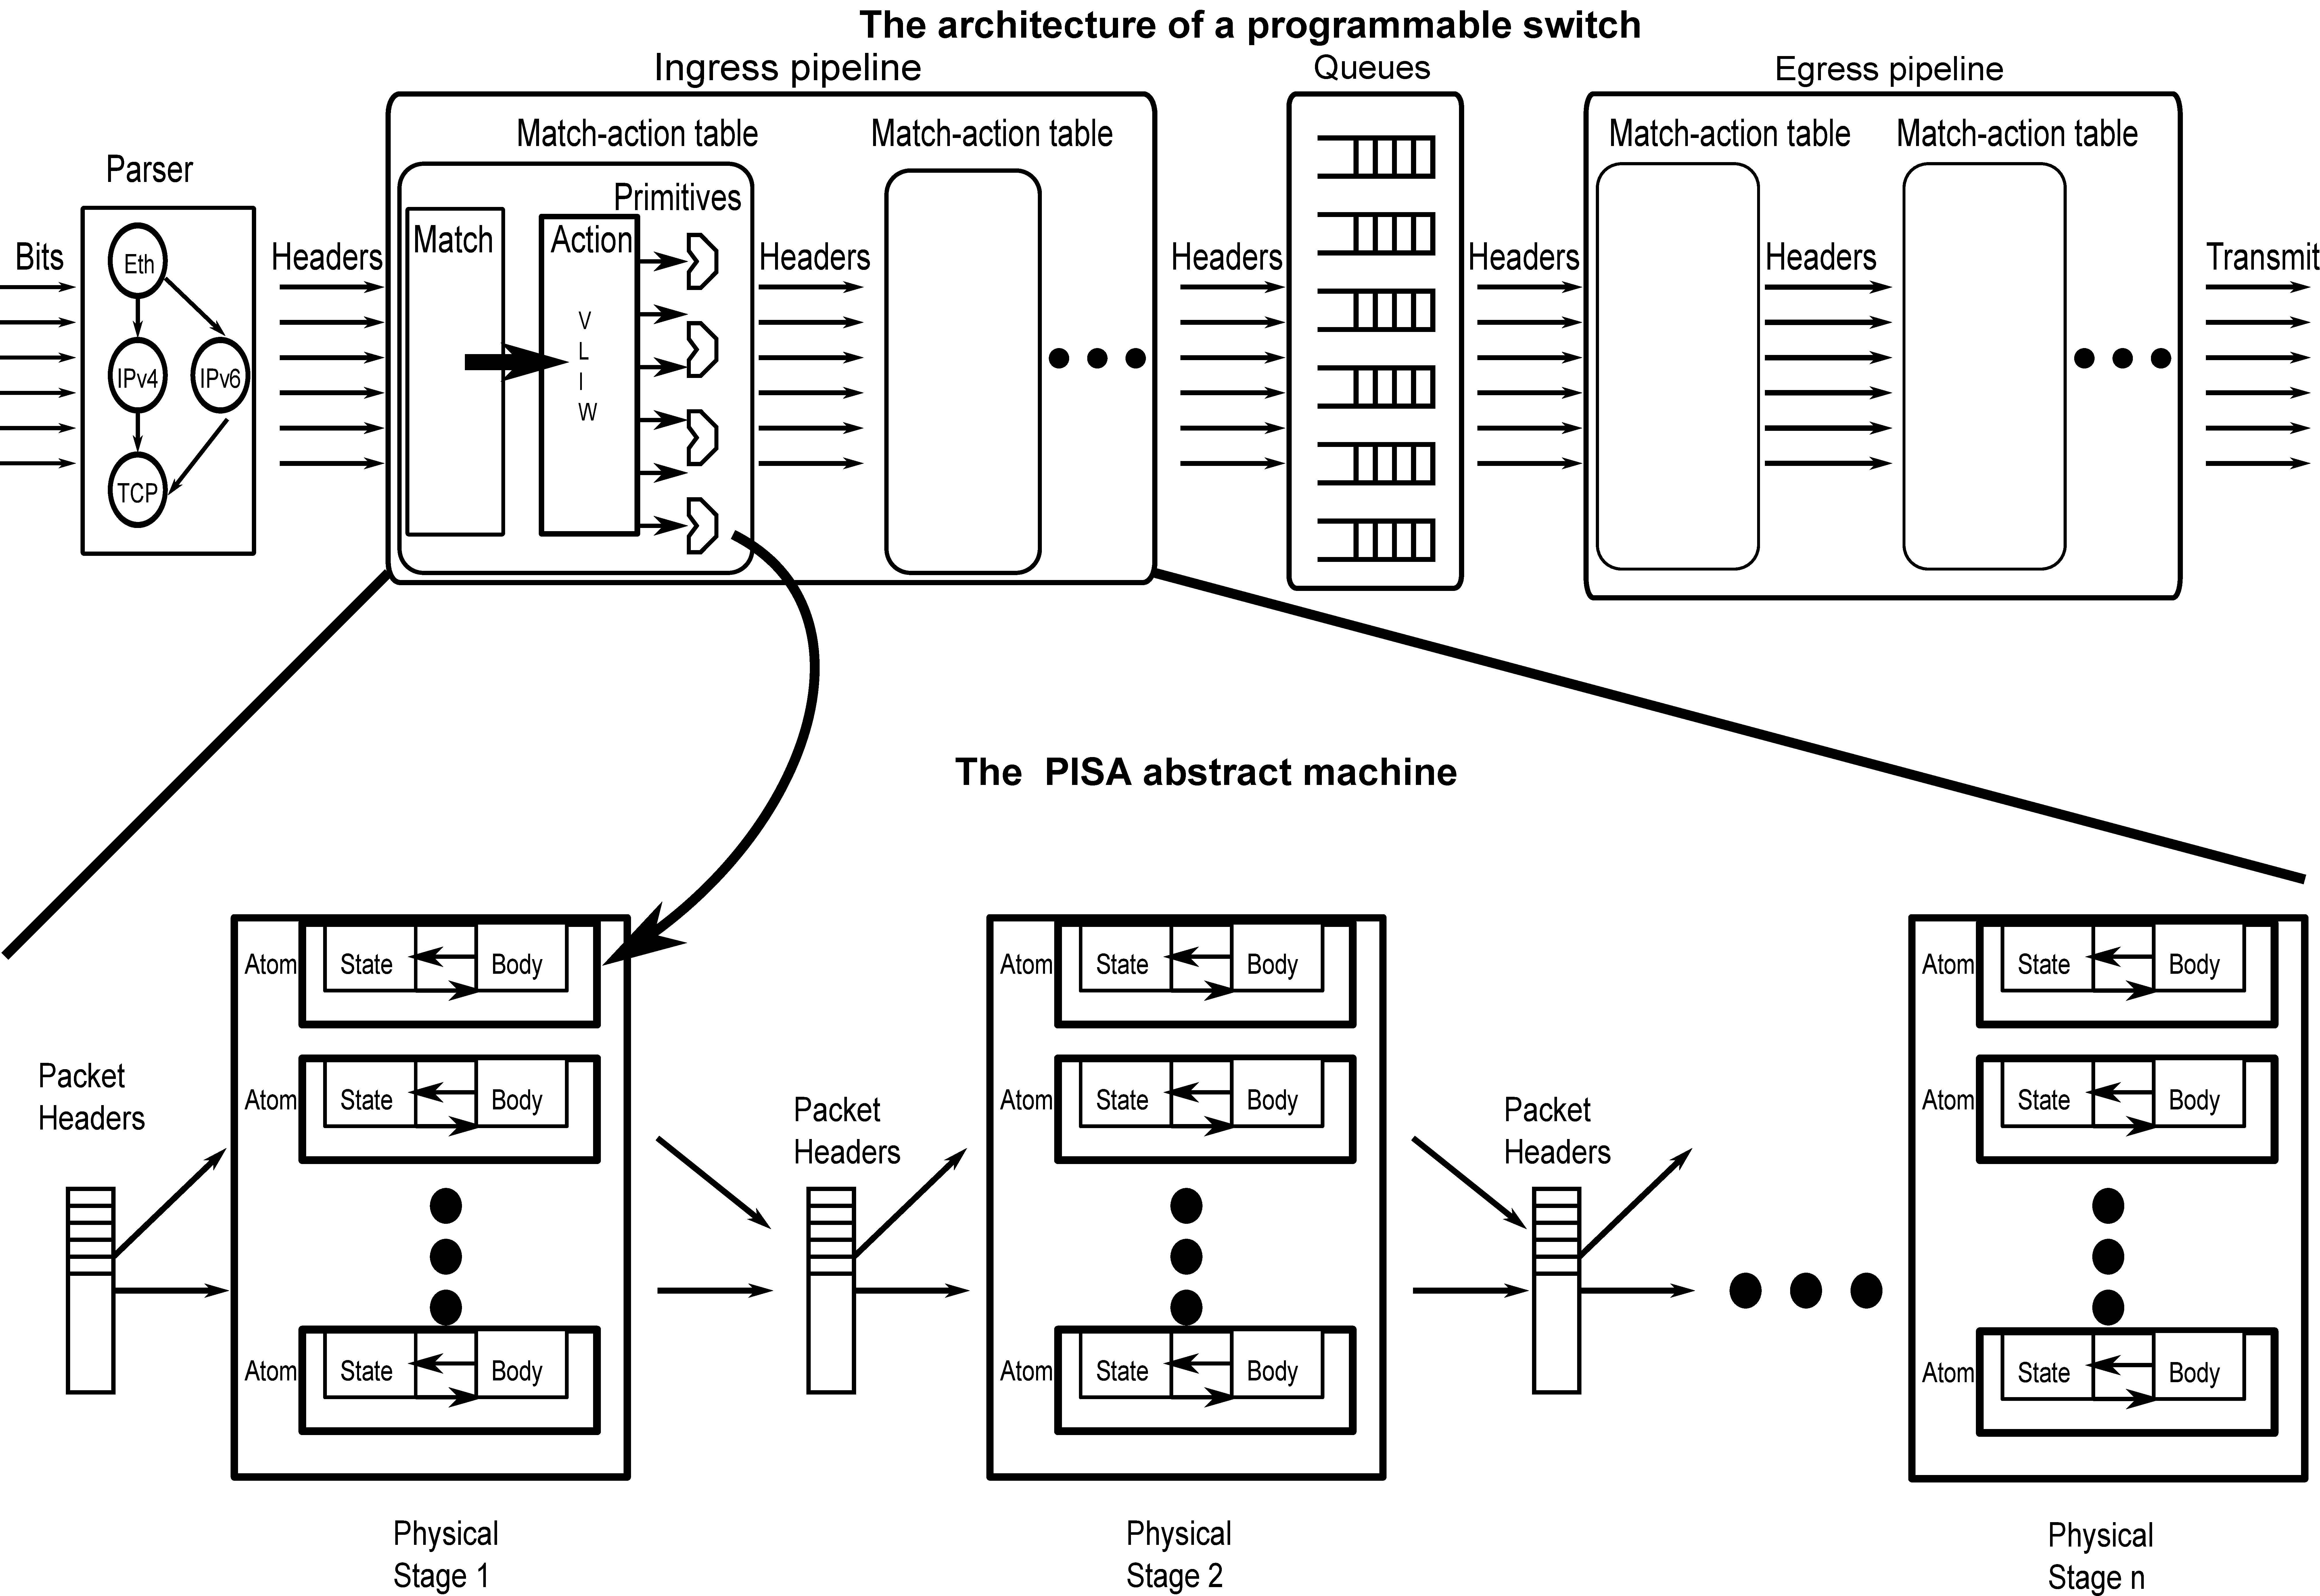
\includegraphics[width=\textwidth]{pisa.pdf}
  \caption{The \absmachine abstract machine and its relationship to
  programmable switch architectures.}
  \label{fig:switch}
\end{figure*}
% deterministic performance or line-rate performance??

We first describe \absmachine, a family of abstract machines that serve as
compiler targets for \pktlanguage. PISA stands for Protocol-Independent Switch
Architecture and was first sketched in a workshop talk~\cite{nick_p4}. Here,
we go further, by describing an executable machine model that serve as a family
of compiler targets for \pktlanguage.

\absmachine is inspired by recent programmable switch architectures with
line-rate performance, such as the Reconfigurable Match-Action Table (RMT)
architecture~\cite{rmt}, Intel's FlexPipe~\cite{flexpipe} architecture, and
Cavium's XPliant Packet architecture~\cite{xpliant}. These architectures assume
the switch model at the top of Figure~\ref{fig:switch}.

Packets arriving to the switch are parsed by a programmable parser that turns
packets into a set of header fields. The set of packet headers is first
processed by an ingress pipeline consisting of match-action tables arranged in
stages. Following the ingress pipeline, the packet is queued, and once it is
dequeued by the switch scheduler, it is processed by a similar egress pipeline
before being transmitted from the switch.

\absmachine models a switch pipeline such as the ingress or egress pipeline. A
pipeline consists of a number of pipeline stages that execute synchronously on
every time step. Each stage is assumed to have one time step of latency;
the inverse of this time step is the line rate supported by the pipeline. Once
a pipeline stage processes a packet, it hands it off to the next pipeline
stage.

As an abstract machine, \absmachine only models the components that are
critical to mapping data-plane algorithms. In particular, it models the
computation that happens in a match-action table in a stage (i.e. the action
half of the match-action table), but not the match semantics (e.g., direct,
ternary, or longest prefix). \absmachine also does not model packet parsing and
assumes that packets arriving to it are already parsed.

\subsection{Atoms: \absmachine's processing units}

Each pipeline stage contains a vector of \textit{atoms}, with the atoms
executing in parallel. Informally, an atom is an atomic unit of packet
processing provided natively by a \absmachine machine and is represented
as a body of imperative code that executes sequentially. An atom is assumed to
complete execution and modify a packet before the next packet is processed by
that atom.

An atom may also contain internal state that persists across packets and
influences the atom's behavior from one packet to the next. For instance, a
switch counter could be written as an atom as follows.\footnote{We use the
  notation p.x to represent access to field ``x'' within a packet p and the
  notation x to represent access to the state variable ``x'' that persists across packets}
  \begin{lstlisting}[style=customc]
  p.tmp     = counter;
  p.tmp2    = p.tmp + 1;
  counter   = p.tmp2;
  \end{lstlisting}
Similarly, a stateless operation that sets a packet field (such as P4's
modify\_field primitive~\cite{p4spec}) can be written as the atom
below:
\begin{lstlisting}[style=customc]
p.field   = value;
\end{lstlisting}

\absmachine generalizes several aspects of existing programmable switch
architectures. The vector of atoms in each stage generalizes RMT's very-large
instruction-word (VLIW)~\cite{rmt} that executes primitive actions on
independent packet fields in parallel. The presence of internal state in an
atom models persistent switch state residing on a switch such as meters,
counters, and P4's register abstraction in a unified manner.

\subsection{Constraining atoms}
\absmachine assumes a synchronous pipeline where each atom executes on every
time step, reading from packet fields at the beginning of the time step and
writing to packet fields at the end of the time step. Because all writes happen
simultaneously at the end of a time step, \absmachine forbids two atoms in the
same stage from writing to the same packet field to avoid dealing with data
races.

To provide deterministic performance at line rate, atoms must be suitably
constrained.  We impose two such constraints that distinguish \absmachine from
software routers such as Click~\cite{click} and network processors such as the
Intel IXP~\cite{ixp4xx} that tradeoff deterministic performance for
increased programmability.

First, \absmachine machines are \textit{shared-nothing}: state variables are
internal to a particular atom and their values can only be communicated to
atoms in subsequent stages by writing them into packet fields that are read
downstream.  This restriction reflects the capabilities of most switches today:
accessing shared memory from multiple switch stages is technically challenging
because it requires multi-ported RAMs and routing long wires on the chip.

Second, we constrain the complexity of atoms by defining {\it atom templates}.
Informally, an atom template is a program that is guaranteed to terminate and
specifies how atoms are executed. One example of a template is an in-order CPU
that can execute exactly $N$ instructions, each with a specific format. Another
is an ALU with a restricted set of primitive operations to choose from. Atom
templates allow us to create different \absmachine machines that support
different atoms natively.

These two atom templates are not exhaustive: as programmable switches evolve,
we expect the computational capabilities of atoms to evolve as well. However,
atoms cannot be arbitrarily complex: a programmable switch's line rate is
inversely proportional to the maximum execution latency of all its atoms.
